


\section{Grundbegriffe der Graphentheorie}

\begin{defn}
Sei $V$ eine endliche Menge und sei $A$ eine Teilmenge von $V \times V$.
Das Paar $D=(V,A)$ heißt \emph{Digraph} (engl.~\emph{directed graph}) mit \emph{Knotenmenge} $V$ und \emph{Kantenmenge}~$A$.
Die Elemente von $V$ heißen \emph{Knoten} und die Elemente von $A$ heißen \emph{(gerichtete) Kanten} (engl.~\emph{arcs}) von~$D$.
Ist $(a,b) \in A$ eine \emph{Kante}, so nennen wir~$a$ ihren \emph{Startknoten} und~$b$ ihren \emph{Endkonten}.
Man sagt auch, dass die Knoten $a$ und $b$ \emph{benachbart} und die Kante $(a,b)$ \emph{inzident} zu~$a$ und $b$ ist.
Eine Kante der Form $(a,a)$ heißt \emph{Schlinge}.
\end{defn}

\begin{bsp} 
Digraphen lassen sich auf vielfache Weise anschaulich darstellen.
Eine verbreitete und nützliche Möglichkeit ist das \glqq Zeichnen\grqq\ in die Ebene.
Ein Digraph mit Doppelkante zwischen den Knoten $1$ und $3$ und Schlinge um den Knoten $7$ sei zum Beispiel wie folgt dargestellt:

\begin{center}
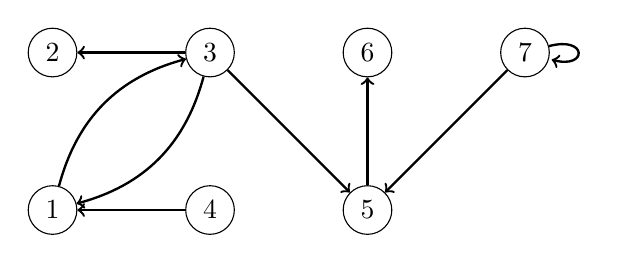
\begin{tikzpicture}[]
 \node[circle,draw=black] (1) at (0,0) {$1$};
 \node[circle,draw=black] (2) at (0,2) {$2$};
 \node[circle,draw=black] (3) at (2,2) {$3$};
 \node[circle,draw=black] (4) at (2,0) {$4$};
 \node[circle,draw=black] (5) at (4,0) {$5$};
 \node[circle,draw=black] (6) at (4,2) {$6$};
 \node[circle,draw=black] (7) at (6,2) {$7$};
		
 \draw[->,line width=0.3mm] (4) edge (1) (3) edge (2) (3) to[bend left] (1) (3) edge (5) (5) edge (6) (7) edge (5);
 \draw[->,line width=0.3mm] (1) to[bend left] (3) (7) edge[loop right] (7);
\end{tikzpicture}
\end{center}
\end{bsp} 

\begin{defn}
Für einen gegebenen Knoten $a \in V$ heißt die Anzahl der Knoten $b \in V$ mit $(a,b) \in A$ der \emph{Ausgangsgrad} von~$a$.
Analog heißt für $b \in V$ die Anzahl der Knoten $a \in V$ mit $(a,b) \in A$ der \emph{Eingangsgrad} von~$b$.
\end{defn} 

\begin{defn}
Sind $D=(V,A)$ und $D'=(V',A')$ zwei Digraphen, so dass $V' \subseteq V$ und $A' \subseteq A$ gelten, so nennt man $D'$ einen \emph{Teilgraphen} von~$D$.
Ist $W \subseteq V$ so heißt
\[
D_{W} := \left( W, \setcond{(a,b)}{a,b \in W \text{ und } (a,b) \in A} \right)
\]
der durch $W$ \emph{induzierte} Teilgraph von~$D$.
\end{defn}

\begin{defn} 
Für einen Digraphen $D=(V,A)$ und Knoten $a,b \in V$ heißt ein Tupel $(v_0,\ldots,v_k)$ mit $(v_i,v_{i+1}) \in A$, für $0 \leq i \leq k-1$ und $v_0=a$ und $v_k=b$ ein \emph{$(a,b)$-Pfad} der Länge~$k$.
Ein Pfad heißt \emph{Weg}, wenn die Knoten des Pfades paarweise verschieden sind.
Der Pfad $(v_i,\ldots,v_j)$ mit $0 \le i \le j \le k$ heißt \emph{Teilpfad} von $(v_0,\ldots,v_k)$.
Ein $(a,b)$-Pfad mit $a=b$ heißt \emph{Zyklus}.
Ein Zyklus $(v_0,\ldots,v_k)$ heißt \emph{Kreis}, falls die Knoten $v_1,\ldots,v_{k-1}$ paarweise verschieden sind.
Die Zyklen $(v_0,\ldots,v_k)$ und $(v_i,\ldots,v_k,v_0,\ldots,v_i)$ werden als gleich angesehen.
Man sagt eine Kante $(u,v)$ \emph{gehört} zu einem Pfad $(v_0,\ldots,v_k)$, falls $u=v_i$ und $v=v_{i+1}$ für ein $i$ mit $0 \le i \leq k-1$ gilt.
Digraphen ohne Zyklen heißen \emph{azyklisch}.
\end{defn} 

%Seien $G=(V,E)$ und $G=(V',E')$ Digraphen und sei $f: V \to V'$ eine Bijektion mit $(a,b) \in E$ $\Leftrightarrow$ $(f(a), f(b)) \in E'$. Die Bijektion $f$ heißt Isomorphismus von $G$ nach $G'$. Zwei Digraphen heißen isomorph, falls ein Isomorphismus von $G$ nach $G'$ existiert. 

\begin{bsp} 
Im Beispieldigraphen von oben markieren wir den Weg $(4,1,3,5,6)$ in blau:

\begin{center}
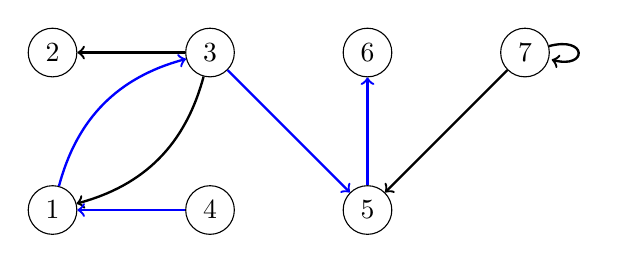
\begin{tikzpicture}[]
 \node[circle,draw=black] (1) at (0,0) {$1$};
 \node[circle,draw=black] (2) at (0,2) {$2$};
 \node[circle,draw=black] (3) at (2,2) {$3$};
 \node[circle,draw=black] (4) at (2,0) {$4$};
 \node[circle,draw=black] (5) at (4,0) {$5$};
 \node[circle,draw=black] (6) at (4,2) {$6$};
 \node[circle,draw=black] (7) at (6,2) {$7$};
		
 \draw[->,line width=0.3mm] (3) edge (2) (3) to[bend left] (1) (7) edge (5);
 \draw[->,line width=0.3mm] (7) edge[loop right] (7);
 \draw[->,line width=0.3mm,blue] (4) edge (1) (1) to[bend left] (3) (3) edge (5) (5) edge (6);
 
\end{tikzpicture}
\end{center}
\end{bsp} 

\begin{bem}
Ein wichtiger Aspekt von Digraphen ist die Orientierung der Kanten, die es ermöglicht zwischen Start- und Endknoten zu unterscheiden.
Wird eine solche Orientierung nicht benötigt, so vereinfachen sich manche Begriffe und wir sprechen anstelle von Digraphen dann von Graphen.
\end{bem} 

\begin{defn} 
Sei dazu $V$ wieder eine endliche Menge und sei $E$ nun eine Teilmenge der ungeordneten Paare $\binom{V}{2}:= \setcond{\{a,b\}}{a, b \in V, a \ne b} $ von Elementen aus~$V$.
Das Paar $G=(V,E)$ heißt \emph{Graph} mit \emph{Knotenmenge} $V$ und \emph{Kantenmenge}~$E$.
Die Elemente von $V$ heißen wieder \emph{Knoten} und die Elemente von $E$ heißen \emph{Kanten} (engl.~\emph{edges}) von~$G$.
Ist $\{a,b\} \in E$ eine Kante, so nennen wir~$a$ und~$b$ ihre \emph{Endknoten}.
Wiederum sagen wir, dass die Knoten $a$ und $b$ \emph{benachbart} und die Kante $\{a,b\}$ \emph{inzident} zu~$a$ und $b$ ist.
\end{defn} 

\begin{bem}
Im Gegensatz zu Digraphen erlaubt die Definition eines Graphen keine Schlingen oder parallele Kanten.
In manchen Literaturquellen lässt man mitunter Mehrfachkanten oder \glqq ungerichtete Schlingen\grqq\ zu und spricht dann von einem \emph{einfachen Graphen} wenn man beides verbietet.
\end{bem}

\begin{defn} 
Für einen Knoten $a \in V$ heißt die Anzahl der Knoten $b \in V$ mit $\{a,b\} \in E$ der \emph{Grad} des Knotens~$a$.
Die Begriffe \emph{(induzierter) Teilgraph}, \emph{Pfad}, \emph{Weg}, \emph{Teilpfad}, \emph{Zyklus} und \emph{Kreis} werden für Graphen analog zu denen für Digraphen definiert.
Ein Graph ohne Zyklen heißt \emph{Wald}.
\end{defn}

\begin{defn} 
Ein Graph $G=(V,E)$ heißt \emph{zusammenhängend}, falls für alle Knoten $a, b \in V$ ein $(a,b)$-Pfad existiert.
Ein zusammenhängender Wald heißt \emph{Baum}.
Die Relation \glqq es existiert ein $(a,b)$-Pfad\grqq\ ist eine Äquivalenzrelation auf den Knoten des Graphen~$G$.
Die Äquivalenzklassen bezüglich dieser Relation heißen \emph{Zusammenhangskomponenten} des Graphen.
Ein Wald ist ein Graph bei dem jede Zusammenhangskomponente ein Baum ist.
\end{defn} 


\begin{bsp}
Die folgende Abbildung zeigt einen Graphen mit zwei Zusammenhangskomponenten:

\begin{center}
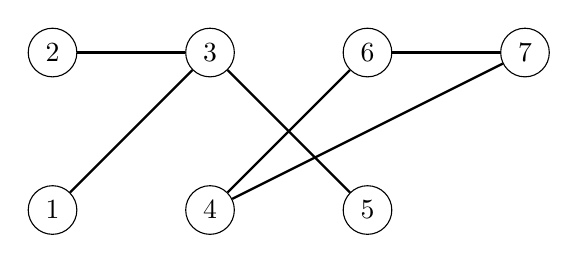
\begin{tikzpicture}[]
 \node[circle,draw=black] (1) at (0,0) {$1$};
 \node[circle,draw=black] (2) at (0,2) {$2$};
 \node[circle,draw=black] (3) at (2,2) {$3$};
 \node[circle,draw=black] (4) at (2,0) {$4$};
 \node[circle,draw=black] (5) at (4,0) {$5$};
 \node[circle,draw=black] (6) at (4,2) {$6$};
 \node[circle,draw=black] (7) at (6,2) {$7$};
		
 \draw[-,line width=0.3mm] (3) edge (2) (3) edge (1) (3) edge (5);
 \draw[-,line width=0.3mm] (4) edge (6) (6) edge (7) (7) edge (4);
\end{tikzpicture}
\end{center}
\end{bsp} 

\begin{bem}
Wir benutzen gelegentlich die Kurzbezeichnung $ab:=(a,b)$ für Kanten von Digraphen und $ab:=\{a,b\}$ für Kanten von Graphen.
Beachten Sie, dass es im Fall einer gerichteten Kante auf die Reihenfolge der Knoten~$a$ und $b$ ankommt.
\end{bem}

\begin{defn}
Ein schleifenfreier Digraph $D = (V,A)$ kann auch als Orientierung eines ungerichteten Graphen $G=(V,E)$ mit $E = \{\{u,v\} : (u,v) \in A\}$ verstanden werden.
Der Graph~$G$ wird dann als der \emph{zugrundeliegende Graph} von~$D$ bezeichnet.
Sobald $E$ nicht leer ist, gibt es stets mindestens zwei Digraphen, denen~$G$ zugrundeliegt.
\end{defn} 

\begin{bsp}
Die folgende Abbildung zeigt einen (schleifenfreien) Digraphen und den dazugehörigen zugrundeliegenden Graphen:
\begin{center}
\hfill
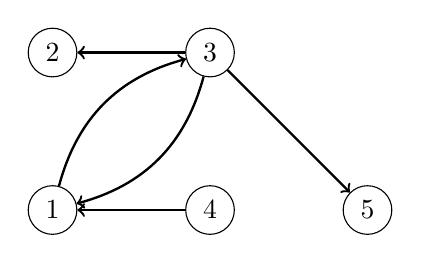
\begin{tikzpicture}[]
 \node[circle,draw=black] (1) at (0,0) {$1$};
 \node[circle,draw=black] (2) at (0,2) {$2$};
 \node[circle,draw=black] (3) at (2,2) {$3$};
 \node[circle,draw=black] (4) at (2,0) {$4$};
 \node[circle,draw=black] (5) at (4,0) {$5$};
		
 \draw[->,line width=0.3mm] (4) edge (1) (3) edge (2) (3) to[bend left] (1) (3) edge (5);
 \draw[->,line width=0.3mm] (1) to[bend left] (3);
\end{tikzpicture}
\hfill
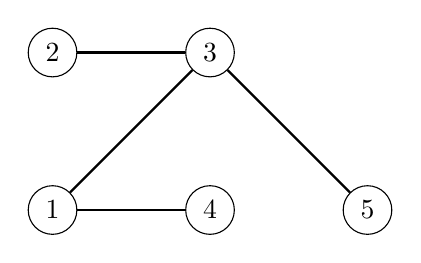
\begin{tikzpicture}[]
 \node[circle,draw=black] (1) at (0,0) {$1$};
 \node[circle,draw=black] (2) at (0,2) {$2$};
 \node[circle,draw=black] (3) at (2,2) {$3$};
 \node[circle,draw=black] (4) at (2,0) {$4$};
 \node[circle,draw=black] (5) at (4,0) {$5$};
		
 \draw[-,line width=0.3mm] (1) edge (4) (3) edge (2) (3) edge (1) (3) edge (5);
\end{tikzpicture}
\hfill\,
\end{center}
Beachten Sie, dass die beiden in entgegengesetzten Richtungen orientierten Kanten zwischen den Knoten $1$ und $3$ zu \emph{einer} Kante im ungerichteten Graphen verschmelzen.
\end{bsp}

\begin{defn} 
Halten wir noch ein paar wichtige spezielle Graphenklassen und deren Bezeichnungen fest: Sei dazu im Folgenden $G=(V,E)$ ein Graph mit $n$ Knoten und $m$ Kanten.
\begin{itemize}
 \item Ist $E=\binom{V}{2}$, so heißt $G$ \emph{vollständig}.
 Ein vollständiger Graph mit $n$ Knoten wird oft mit~$K_n$ bezeichnet.

 \item Ist $E=\emptyset$, so heißt $G$ \emph{leer}.
 Ein leerer Graph mit $n$ Knoten wird oft mit~$\bar K_n$ bezeichnet.

 \item Ist $V$ eine disjunkte Vereinigung zweier Mengen $A$ und $B$ und hat jede Kante von~$G$ die Form $\{a,b\}$ mit $a \in A$ und $b \in B$, so heißt $G$ \emph{bipartit}.
 Die Mengen~$A$ und $B$ heißen dann \emph{Partitionsklassen} von $G$.
 
 \item Ist $G$ bipartit und gilt darüber hinaus, dass jedes $\{a,b\}$ mit $a \in A$ und $b \in B$ eine Kante von $G$ ist, so heißt $G$ \emph{vollständig bipartit}.
 Ein vollständig bipartiter Graph, deren Partitionsklassen die Größe~$r$ und~$s$ haben, wird oft mit~$K_{r,s}$ bezeichnet.
 Natürlich gilt $n = r + s$.
 
 \item Eine \emph{Einbettung} von~$G$ in die Ebene~$\R^2$ ist eine Menge $P=\{p_1,\ldots,p_n\} \subseteq \R^2$ von Punkten zusammen mit einer Menge $S=\{S_1,\ldots,S_m\}$ von Streckensegmenten, so dass es eine Bijektion $f:V \to P$ gibt mit der Eigenschaft, dass $\{u,v\}$ genau dann eine Kante von~$G$ ist, wenn die Punkte $f(u)$ und $f(v)$ Eckpunkte desselben Streckensegmentes~$S_i$ sind.
 Besitzt ein Graph eine Einbettung bei der je zwei verschiedene Streckensegmente sich höchstens in Eckpunkten schneiden, so heißt dieser Graph \emph{planar}.
 
 Beispiele: $K_n$ ist planar genau dann wenn $n\leq4$ ist; $K_{3,3}$ ist nicht planar.
\end{itemize}
\end{defn} 

\begin{bsp}
Die nachfolgende Illustration zeigt zwei Darstellungen des $K_4$:
\begin{center}
\hfill
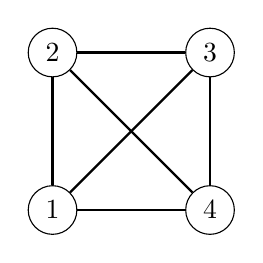
\begin{tikzpicture}[]
\tikzset{every loop/.style={}} % no arrows in loops
 \node[circle,draw=black] (1) at (0,0) {$1$};
 \node[circle,draw=black] (2) at (0,2) {$2$};
 \node[circle,draw=black] (3) at (2,2) {$3$};
 \node[circle,draw=black] (4) at (2,0) {$4$};
		
 \draw[-,line width=0.3mm] (1) edge (2) (1) edge (3) (1) edge (4) (2) edge (3) (2) edge (4) (3) edge (4);
		% (4) edge[loop right] (4);		
\end{tikzpicture}
\hfill
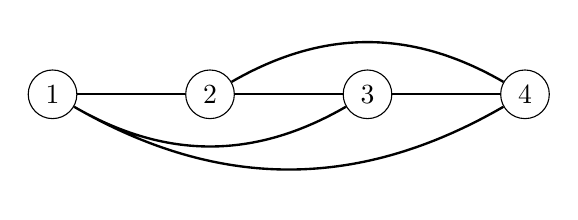
\begin{tikzpicture}[]
\tikzset{every loop/.style={}} % no arrows in loops
 \node[circle,draw=black] (1) at (0,0) {$1$};
 \node[circle,draw=black] (2) at (2,0) {$2$};
 \node[circle,draw=black] (3) at (4,0) {$3$};
 \node[circle,draw=black] (4) at (6,0) {$4$};
		
 \draw[-,line width=0.3mm] (1) edge (2) (2) edge (3) (3) edge (4);
 \draw[-,line width=0.3mm] (1) to[bend right] (3) (1) to[bend right] (4);
 \draw[-,line width=0.3mm] (2) to[bend left] (4);		
\end{tikzpicture}
\hfill\,
\end{center}
Keine der beiden Darstellungen zeigt, dass $K_4$ planar ist.
Warum nicht?
Finden Sie eine Darstellung, die dies illustriert!
\end{bsp}



\begin{bem}
In der Graphentheorie ist die Bezeichnung der Hautbegriffe nicht einheitlich.
Von Quelle zu Quelle unterscheiden sich die Definitionen geringfügig und insbesondere in Bezug auf die Namensgebung gibt es teilweise große Unterschiede.
Zu diesem Zweck listen wir hier die geläufigsten Synonyme um mögliche Verwirrungen beim Lesen unterschiedlicher Quellen zu vermeiden:
\begin{align*}
\text{gerichteter Graph} &= \text{Digraph}\\
\text{Knoten} &= \text{Ecke}\\
\text{gerichtete Kante} &= \text{Bogen}\\
\text{adjazent} &= \text{benachbart}\\
\text{Grad} &= \text{Valenz}\\
\text{Weg} &= \text{einfacher Pfad}\\
\text{Kreis} &= \text{einfacher Zyklus}\\
\text{Kantenzug} &= \text{Pfad}\\
\text{geschlossener Kantenzug} &= \text{Zyklus}\\
\text{Schleife} &= \text{Schlinge}
\end{align*}
\end{bem}

\begin{bem}
Zum Abschluss dieser Einführung in die Grundbegriffe schauen wir uns noch verschiedene Möglichkeiten an, wie man einen gegebenen (Di)Graphen im Rechner darstellt, das heißt, in welcher Form man die Beziehungen zwischen Knoten und (gerichteten) Kanten verwalten kann.

Sei dazu ein Graph oder ein Digraph gegeben und zur Vereinheitlichung im Folgenden mit $G=(V,E)$ bezeichnet.
\end{bem} 

\begin{defn}
{\bfseries Kantenliste:} Liste/Array der Kanten von $G$. 
\end{defn}

\begin{bsp}\ 
\begin{center}
\hfill
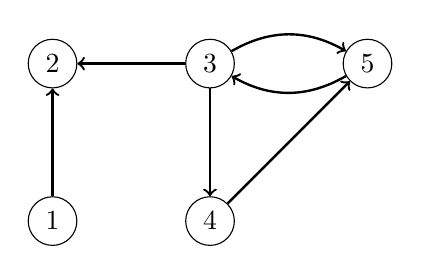
\begin{tikzpicture}[]
 \node[circle,draw=black] (1) at (0,0) {$1$};
 \node[circle,draw=black] (2) at (0,2) {$2$};
 \node[circle,draw=black] (3) at (2,2) {$3$};
 \node[circle,draw=black] (4) at (2,0) {$4$};
 \node[circle,draw=black] (5) at (4,2) {$5$};
% \node[black] (G) at (2,3.5) {$G=(V,E)$};
		
 \draw[->,line width=0.3mm] (1) edge (2) (3) edge (2) (3) edge (4) (3) to[bend left] (5) (4) edge (5);
 \draw[->,line width=0.3mm] (5) to[bend left] (3);
\end{tikzpicture}
\hfill
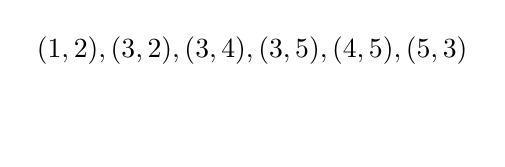
\begin{tikzpicture}[]
 \node[black] (1) at (0,0) {$(1,2),(3,2),(3,4),(3,5),(4,5),(5,3)$};
 \node[black] (1) at (0,-1) {$ $};
\end{tikzpicture}
\hfill\,
\end{center}
\end{bsp}

\begin{defn} 
{\bfseries Adjazenzliste:} Hier speichern wir die Knotenmenge $V$ als Liste und jedem Element $u \in V$ der Liste wird eine Liste aller Knoten $v \in V$ mit $uv \in E$ zugeordnet.
Der Speicherplatzbedarf für diese Darstellung ist offensichtlich $\Theta(|V|+|E|)$.
\end{defn}

\begin{bsp} \ 
\begin{center}
\hfill
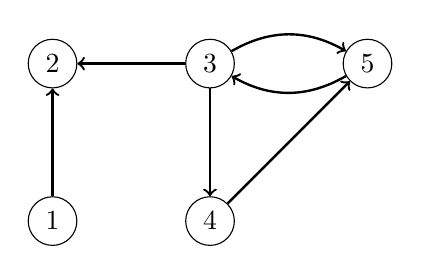
\begin{tikzpicture}[]
 \node[circle,draw=black] (1) at (0,0) {$1$};
 \node[circle,draw=black] (2) at (0,2) {$2$};
 \node[circle,draw=black] (3) at (2,2) {$3$};
 \node[circle,draw=black] (4) at (2,0) {$4$};
 \node[circle,draw=black] (5) at (4,2) {$5$};
% \node[black] (G) at (2,3.5) {$G=(V,E)$};
		
 \draw[->,line width=0.3mm] (1) edge (2) (3) edge (2) (3) edge (4) (3) to[bend left] (5) (4) edge (5);
 \draw[->,line width=0.3mm] (5) to[bend left] (3);
\end{tikzpicture}
\hfill
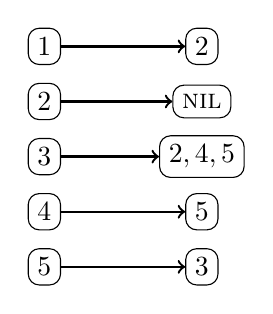
\begin{tikzpicture}[]
 \node[rounded corners,draw=black] (1) at (0,0) {$1$};
 \node[rounded corners,draw=black] (L1) at (2,0) {$2$};
 \node[rounded corners,draw=black] (2) at (0,-.7) {$2$};
 \node[rounded corners,draw=black] (L2) at (2,-.7) {$\textsc{nil}$};
 \node[rounded corners,draw=black] (3) at (0,-1.4) {$3$};
 \node[rounded corners,draw=black] (L3) at (2,-1.4) {$2,4,5$};
 \node[rounded corners,draw=black] (4) at (0,-2.1) {$4$};
 \node[rounded corners,draw=black] (L4) at (2,-2.1) {$5$};
 \node[rounded corners,draw=black] (5) at (0,-2.8) {$5$};
 \node[rounded corners,draw=black] (L5) at (2,-2.8) {$3$};
		
 \draw[->,line width=0.3mm] (1) edge (L1) (2) edge (L2) (3) edge (L3) (4) edge (L4) (5) edge (L5);
\end{tikzpicture}
\hfill\,
\end{center}
\end{bsp} 

\begin{defn} 
{\bfseries Adjazenzmatrix:} Sei $V=\{v_1,\ldots,v_n\}$.
Die Adjazenzmatrix von~$G$ ist die Matrix $A=(a_{i,j}) \in \R^{n \times n}$ mit Einträgen
\[
a_{i,j} = \begin{cases}1&,\text{ falls }\{v_i,v_j\} \in E \text{ bzw.~falls }(v_i,v_j) \in E,\\ 0&,\text{ sonst}.\end{cases}
\]
Der Speicherplatzbedarf (bei direkter Implementierung von Matrizen) ist $\Theta(|V|^2)$.

\begin{center}
\hfill
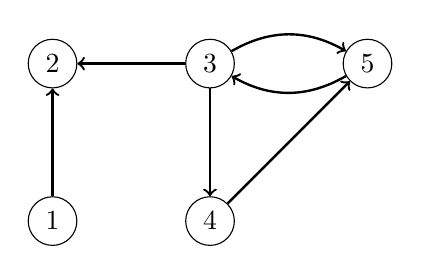
\begin{tikzpicture}[]
 \node[circle,draw=black] (1) at (0,0) {$1$};
 \node[circle,draw=black] (2) at (0,2) {$2$};
 \node[circle,draw=black] (3) at (2,2) {$3$};
 \node[circle,draw=black] (4) at (2,0) {$4$};
 \node[circle,draw=black] (5) at (4,2) {$5$};
% \node[black] (G) at (2,3.5) {$G=(V,E)$};
		
 \draw[->,line width=0.3mm] (1) edge (2) (3) edge (2) (3) edge (4) (3) to[bend left] (5) (4) edge (5);
 \draw[->,line width=0.3mm] (5) to[bend left] (3);
\end{tikzpicture}
\hfill
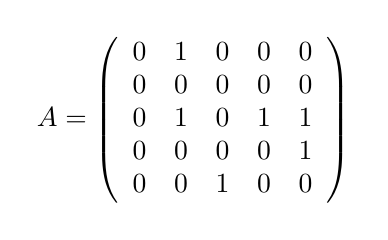
\begin{tikzpicture}[]
 \node[black] (1) at (0,0) {$A=\left(\begin{array}{ccccc}
0 & 1 & 0 & 0 & 0 \\
0 & 0 & 0 & 0 & 0 \\
0 & 1 & 0 & 1 & 1 \\
0 & 0 & 0 & 0 & 1 \\
0 & 0 & 1 & 0 & 0
\end{array}\right)$
};
\end{tikzpicture}
\hfill\,
\end{center}
\end{defn} 

\begin{defn}
{\bfseries Inzidenzmatrix:} Sei $V=\{v_1,\ldots,v_n\}$ und $E=\{e_1,\ldots,e_m\}$.
Sei weiterhin $G$ zunächst als gerichteter Graph ohne Schleifen angenommen.
Die Inzidenzmatrix von~$G$ ist die Matrix $B=(b_{i,j}) \in \R^{n \times m}$ mit Einträgen
\[
b_{i,j} = \begin{cases}1&,\text{ falls }v_i\text{ Startknoten von }e_j\text{ ist},\\ -1&,\text{ falls }v_i\text{ Endknoten von }e_j\text{ ist},\\ 0&,\text{ sonst}.\end{cases}
\]
Ist $G$ ein ungerichteter Graph, so lassen wir lediglich die Vorzeichen weg, das heißt, die Einträge der Inzidenzmatrix sind
\[
b_{i,j} = \begin{cases}1&,\text{ falls }v_i\text{ Endknoten von }e_j\text{ ist},\\ 0&,\text{ sonst}.\end{cases}
\]
Der Speicherplatzbedarf (bei direkter Implementierung von Matrizen) ist $\Theta(|V|\cdot|E|)$.
\end{defn} 

\begin{bsp} \ 
\begin{center}
\hfill
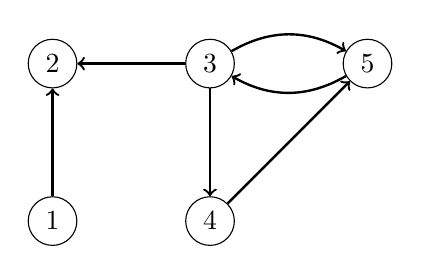
\begin{tikzpicture}[]
 \node[circle,draw=black] (1) at (0,0) {$1$};
 \node[circle,draw=black] (2) at (0,2) {$2$};
 \node[circle,draw=black] (3) at (2,2) {$3$};
 \node[circle,draw=black] (4) at (2,0) {$4$};
 \node[circle,draw=black] (5) at (4,2) {$5$};
% \node[black] (G) at (2,3.5) {$G=(V,E)$};
		
 \draw[->,line width=0.3mm] (1) edge (2) (3) edge (2) (3) edge (4) (3) to[bend left] (5) (4) edge (5);
 \draw[->,line width=0.3mm] (5) to[bend left] (3);
\end{tikzpicture}
\hfill
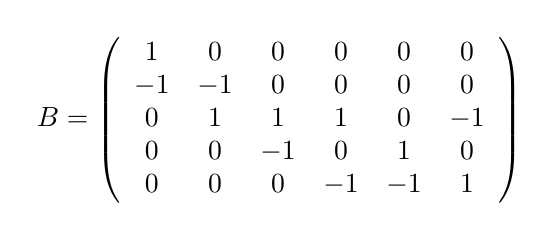
\begin{tikzpicture}[]
 \node[black] (1) at (0,0) {$B=\left(\begin{array}{cccccc}
1 & 0 & 0 & 0 & 0 & 0\\
-1 & -1 & 0 & 0 & 0 & 0\\
0 & 1 & 1 & 1 & 0 & -1\\
0 & 0 & -1 & 0 & 1 & 0\\
0 & 0 & 0 & -1 & -1 & 1
\end{array}\right)$
};
\end{tikzpicture}
\hfill\,
\end{center}

Die Kanten in der vorigen Abbildung sind in der Reihenfolge $12,32,34,35,45,53$ nummeriert.
\end{bsp} 